\section{Introduction}

In an epidemic, symptomatic cases are the predominant focus of treatment and usually represent the bulk of reported cases. 
However, infected individuals who are asymptomatic yet infectious can be a critical factor in the spread of some pathogens \citep{fraser2004factors}.
Asymptomatic individuals are hard to trace, unlikely to self-isolate, and are likely to retain normal social and travel patterns.

There is significant ongoing interest in asymptomatic infections in COVID-19 for two major reasons~\citep{fauci_nejm2020}. 
First, the proportion of infections that are asymptomatic (see~\citep{mizumoto_2020}) is critical to attempts to estimate the likely burden of severe outcomes (including mortality) when the virus spreads through a population.
Second, understanding the possible role of \emph{transmission} by asymptomatic individuals is crucial to planning surveillance and control efforts.

Here, we focus on a third effect. 
If asymptomatic cases are important for transmission, they also have the potential to affect estimates of key parameters of disease spread such as the basic reproduction number ${\cal{R}}_0$ (i.e., the expected number of secondary cases generated by an average primary case in a fully susceptible population \citep{anderson1992infectious}). 
Thus, we investigate the relationship between individual-level features of asymptomatic cases (e.g., the probability that an infection is asymptomatic, asymptomatic case duration, transmission by asymptomatic individuals) to dynamics at the population scale.

\section{Methods}

We model viral spread using a renewal-equation framework \citep{heesterbeek1996concept}, which allows us to model the current incidence of infected individuals (i.e., the the rate at which new infections occur in the population) as a function of previous incidence and how infectiousness of an infected individual varies over the course of their infection.
We divide incidence $i$ into two categories -- $i_a$ and $i_s$ -- corresponding to incidence of asymptomatic and symptomatic cases, respectively.
Newly infected individuals that are either asymptomatically or symptomatically infected can transmit the disease to others, but they differ in their intrinsic reproduction numbers, ${\cal{R}}_a$ and ${\cal{R}}_s$, respectively, as well as intrinsic generation-interval distributions \citep{champredon2015intrinsic}, $g_a(\tau)$ and $g_s(\tau)$.
Generation intervals, which are defined as the time between when an individual is infected and when that individual infects another person \citep{svensson2007note}, depend on the natural history of infection:
individuals with subclinical infections may have fast clearance and short generation intervals, or slow viral reproduction and long generation intervals (cf. \citep{roberts2007model}).
The shape of the generation-interval distribution characterizes the relationship between the epidemic growth rate $r$ and the reproduction number \citep{wallinga2007generation}.

Neglecting births and loss of immunity on the time scale of the outbreak, the dynamics of susceptibles and incidence are:
\begin{eqnarray}
\dot{S}&=&-i(t) \\
i(t)&=&\mathcal R_a S(t) \int_0^\infty i_a(t-\tau) g_a(\tau) \mathrm{d}\tau + \mathcal R_s S(t) \int_0^\infty i_s(t-\tau) g_s(\tau) \mathrm{d}\tau.
\end{eqnarray}
The basic reproduction number of this system is:
\begin{equation}
{\cal{R}}_{0}= p {\cal{R}}_a + (1-p) {\cal{R}}_s,
\end{equation}
where $p$ is the proportion of \emph{incident cases} that are asymptomatic: $i_a(t) = p i(t)$.
The corresponding intrinsic generation-interval distribution of an average infected individual is given by: 
\begin{equation}
g(\tau) = z g_a(\tau) + (1-z) g_s(\tau),
\end{equation}
where we define the ``intrinsic'' proportion of asymptomatic transmission $z$ as the relative contribution of asymptomatic cases to the basic reproduction number:
\begin{equation}
z = p {\cal{R}}_a/{\cal{R}}_{0}.
\end{equation}
Note that the intrinsic proportion of symptomatic transmission satisfies
\begin{equation}
1-z = (1-p) {\cal{R}}_s/{\cal{R}}_{0}.
\end{equation}
Yet, this information is not sufficient to disentangle the role of asymptomatic cases, i.e., what fraction of secondary cases can be ascribed to \emph{realized} transmission from asymptomatic cases vs.~symptomatic cases?

The intrinsic proporton of asymptomatic transmission $z$ is a useful benchmark, but does not necessarily reflect the realized proportion of asymptomatic transmission, unless both types of infection have the same generation-interval distribution.
The \emph{realized} proportion of asymptomatic transmission, $q$ at time $t$ is given by:
\begin{equation}
\frac{q}{1-q}=\frac{\mathcal R_a S(t) \int_0^\infty i_a(t-\tau) g_a(\tau) \mathrm{d}\tau}{\mathcal R_s S(t) \int_0^\infty i_s(t-\tau) g_s(\tau) \mathrm{d}\tau},
\end{equation}
During the period of exponential growth, we assume $S$ remains nearly constant, and $i(t)$ is proportional to $\exp(r t)$, and simplify: 
\begin{equation}
\frac{q}{1-q}=\left(\frac{z}{1-z}\right)\frac{\delta_a}{\delta_s}.
\label{eq.qratio}
\end{equation}
Here, $\delta_c$ for each of the two classes is the average ``discount'' of a new infection -- the average relative contribution of a secondary infection to the epidemic, taking exponential growth into account:
\begin{equation}
	\delta_c = \int_0^\infty \exp(-r\tau) g_c(\tau) \mathrm{d}\tau.
\end{equation}
$\delta_c<1$ and grows smaller as the generation interval grows longer.
Thus, the realized proportion of asymptomatic infections will be increased (resp., decreased) if transmission is relatively faster (slower) along the asymptomatic route.
The discount $\delta$ also depends on the relative variation in the generation-interval distribution, the ``dispersion'': more variation in generation intervals leads to more opportunities for fast spread and thus to higher values of $\delta$ (similar to shorter average generation intervals). 

To estimate the effects of assumptions about asymptomatic transmission on the importance of asymptomatic transmission and estimates of the basic reproduction number ${\cal{R}}_0$, we parameterize the generation interval distributions of asymptomatic and symptomatic cases based on their means, $\bar G_a$ and $\bar G_s$, and dispersions, $\kappa_a$ and $\kappa_s$.
We assume that generation intervals are gamma distributed, and we set the dispersion to be equal to the squared coefficient of variation (the reciprocal of the gamma shape parameter, see Appendix).
We assume that epidemic growth rate $r$ and the generation-interval distribution of symptomatic case are known, using parameter values that are consistent with earlier COVID-19 models \citep{park_preprint}: $1/r=7$ days, $\bar G_s=8$ days, and $\kappa_s=0.5$.
We infer values of $q$ using Eq.~\req{eq.qratio} and ${\cal{R}}_0$ using the Euler-Lotka equation:
\begin{equation}
\frac{1}{\mathcal R_0} = \int \exp(-r \tau) g(\tau) \mathrm{d} \tau.
\end{equation}
In the supplementary material, we also use ODEs to give a concrete example of how differences in generation intervals affect both $q$ and estimates of $\mathcal R_0$.

\section{Results}

\begin{figure*}[b!]
\begin{center}
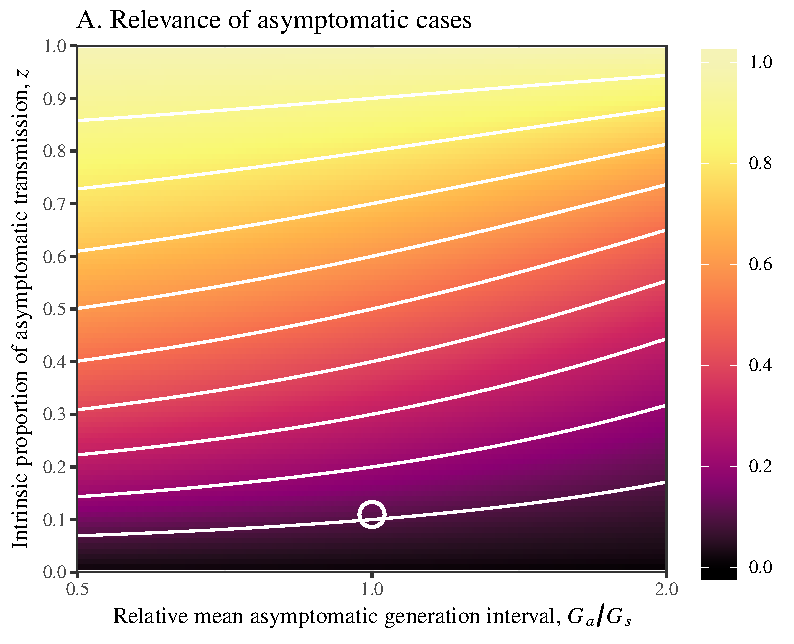
\includegraphics[width=0.4\textwidth]{figheatmap.pdf}
\mbox{\hspace{0.05\textwidth}}
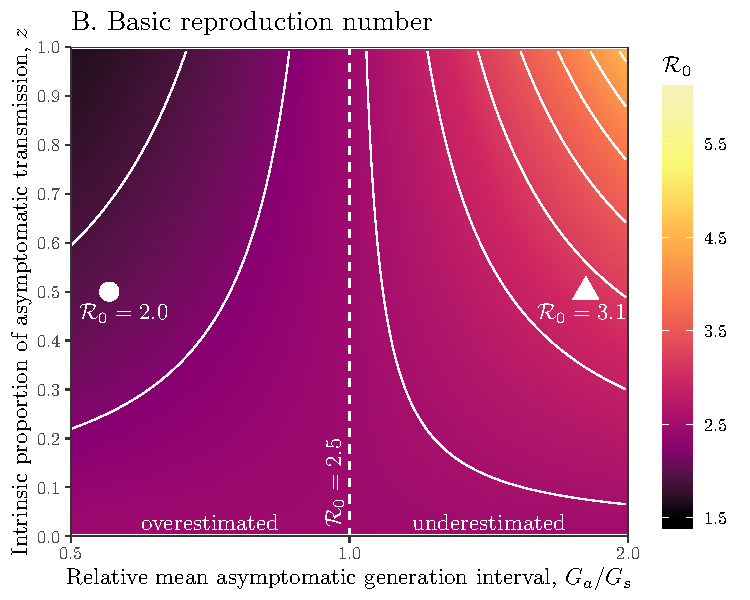
\includegraphics[width=0.4\textwidth]{figheatmap_R0.pdf}
\caption{Effects of intrinsic proportion of asymptomatic transmission on the realized proportion of asymptomatic transmission and basic reproduction number, given variation in
the mean generation interval of asymptomatic cases. 
(A) Increasing the speed of asymptomatic transmission (shorter generation intervals) increases the importance of asymptomatic cases in transmission, $q$.
(B) Increasing generation intervals of asymptomatic cases increases the basic reproduction number ${\cal{R}}_0$; 
When $\bar G_a$ is smaller (larger) than $\bar G_s$, estimates based on the observed generation distribution for symptomatic cases (dashed line) are expected to over- (under-) estimate the true $\mathcal R_0$.
Solid lines show contours for \Ro\ values. 
Here, we assume $1/r=7$ days, $\bar G_s=8$ days, and $\kappa_s=\kappa_a=0.5$.
\label{fig.importance}}
\end{center}
\end{figure*}

We explore the effects of different assumptions about speed and effectiveness of asymptomatic transmission on the importance of asymptomatic transmission and estimates of the basic reproduction number ${\cal{R}}_0$, using a gamma assumption (see Methods).
Across the range of parameters we explore, the intrinsic proportion of asymptomatic transmission $z$ is similar to the realized proportion $q$ (Figure~\ref{fig.importance}A).
As the relative mean generation interval of asymptomatic transmission, $\bar G_a/\bar G_s$, increases, $q$ decreases because symptomatic cases are more likely to have short generation intervals (i.e., fast transmission events), which drive the spread during the growth phase (Figure~\ref{fig.importance}A).

Figure~\ref{fig.importance}B shows the effect of different assumptions about the generation interval of asymptomatic cases, $\bar G_a$, on the basic reproduction number ${\cal{R}}_0$.
When $\bar G_a$ is long compared to $\bar G_s$, then we are effectively assuming a longer mean for the overall generation interval. 
This assumption leads to a larger estimate of \Ro\ for i fixed value of $r$. (see~\citep{park_2019practical}).
Conversely, when $\bar G_a < \bar G_s$, generation intervals are shorter, leading to lower estimates of the epidemic strength \Ro. Both of these effects are stronger when the intrinsic proportion of asymptomatic transmission $z$ increases (and disappear as $z\to0$).
Therefore, when ${\cal{R}}_0$ is estimated without explicitly accounting for asymptomatic spread (white, dashed line in Figure~\ref{fig.importance}B), it can be over- or under- estimated depending on the relative duration of infection between symptomatic and asymptomatic individuals.
The qualitative effects of $z$ and $\bar G_a/\bar G_s$ on $q$ and ${\cal{R}}_0$ remain robust when we assume narrower ($\kappa_s = \kappa_a = 0.3$; Figure~S1) or wider ($\kappa_s = \kappa_a = 0.8$; Figure~S2) generation intervals.

Relative generation-interval dispersion of asymptomatic cases $\kappa_a/\kappa_s$ have similar, but smaller, effects on $q$ and ${\cal{R}}_0$ (Figure~S3).
Since a wider generation-interval distribution has a higher proportion of early transmission than a narrow one, increasing the generation-interval dispersion has qualitatively similar effects on $q$ and ${\cal{R}}_0$ as decreasing the mean generation interval.

\section{Discussion}

Much is still unknown about course of asymptomatic infection compared to symptomatic infection in COVID-19. 
Our current work highlights the need to characterize the duration of asymptomatic infections, relative to that of symptomatic ones, and their consequences not only for contact tracing but for precise estimation of the basic reproduction number of the ongoing COVID-19 outbreak~\citep{park_preprint}.
The present findings are also consistent with a recent generalization linking speed, strength, and generation intervals, such that for a given observed speed increases in the mean generation interval imply larger reproduction number~\citep{park_2019practical}.

If mild, asymptomatic infections are more persistent than severe, symptomatic ones, the mean generation interval for COVID-19 could be longer than estimated from symptomatic cases alone - possibly increasing ${\cal{R}}_0$ (Figure~\ref{fig.importance}B).
However, if asymptomatic cases tend to have shorter infection, then current estimates of ${\cal{R}}_0$ may be over-estimates of the underlying strength (Figure~\ref{fig.importance}B), although asymptomatic cases may be driving a larger fraction of secondary cases than we would expect without accounting for their differences (Figure~\ref{fig.importance}A).
Therefore, current estimates of ${\cal{R}}_0$ that do not account for asymptomatic cases may be systematically biased.

Finally, it is important to note we focused here on the exponential phase, but that the realized proportion of asymptomatic transmission $q$ is time-dependent, and will vary given the population state structure of infected individuals. Such variation in the ratio of asymptomatic to symptomatic cases will also impact estimates of case fatality rates insofar as many asymptomatic cases are not counted, particularly early in an outbreak.
Future work might also consider the ways in which asymptomatic individuals modulate resurgent epidemics in a networked metapopulation~\citep{watts_pnas2005}.
Characterizing the role of asymptomatic individuals in driving the persistence of the epidemic will be critical for assessing the post-pandemic outcome \citep{lipsitch_preprint}.

%We also note that efforts to characterize asymptomatic tranissmion
%should consider its effect on
%the basic reproduction number, which for this SEIR coronavirus-like model is ${\cal{R}}_0=p\left(\frac{\beta_a}{\gamma_a}\right)+ (1-p)\left(\frac{\beta_s}{\gamma_s}\right).$
%%Pooling estimates via a Bayesian approach applied to the early stages of Wuhan case data,
%%suggests ${\cal{R}}_0\approx 3.0$ 
%%with a 95\% confidence interval from 2-4.5.  Yet, that information
%%is not sufficient to disentangle the role of asymptomatic cases, i.e.,
%%what fraction of secondary cases can be ascribed to transmission
%%from asymptomatic cases vs.~symptomatic cases?  
%Strength, ${\cal{R}}_0$ and size $r$
%can be related via a Gamma approximation to the generation
%interval distribution as follows:
%\begin{equation}
%{\cal{R}}^{gamma}=(1+\kappa r \bar{G})^{1/\kappa}
%\end{equation}
%where $\bar{G}$ is the mean generation interval and
%$\kappa$  is the squared coefficient of variation of
%the generation interval.  
%This approximation (explored in Champredon
%et al.) reveals why for a given observed speed,
%increases in the mean generation interval imply
%larger reproduction number. Hence, reports of individuals
%with mild cases that remain infectious for (relatively)
%long periods suggest that the mean generation interval
%could be longer than estimated from symptomatic cases alone - both
%increasing ${\cal{R}}_0$ and driving a larger fraction of secondary cases.
%This inference also reinforces 
%the need to characterize the epidemiological characteristics of asymptomatic transmission.

%Renewal equations provide a route to connect
%observed increases in case counts, i.e.,
%\begin{equation}
%{\cal{R}}_0 = \frac{1}{M(-r)}
%\end{equation}
%where $r$ is the speed of the disease spread and $M(r)$ is the
%moment generating function of the generation interval distribution
%$g(a)$ (normalized age of transmission) such that 
%\begin{equation}
%M(r)=\int_0^{\infty}\mathrm{d} a e^{ra}g(a).
%\end{equation}
%For the present model, the moment generating function is
%\begin{equation}
%M(r)=qM_E(r)M_{I_a}(r)+(1-q)M_E(r)M_{I_s}(r)
%\end{equation}
%where each of the component functions are $M_E(-r)=\frac{\gamma_e}{\gamma_e+r}$,
%$M_{I_a}(-r)=\frac{\gamma_a}{\gamma_a+r}$, 
%$M_{I_s}(-r)=\frac{\gamma_s}{\gamma_s+r}$,
%and $q$ is the fraction of realized new secondary cases caused by
%asymptomatic individuals. The relevance $q$ is an unknown feature of
%outbreaks at the population scale, distinct from $p$ the probability of having
%an asymptomatic cases, conditional upon being infected
%but not yet infectious. Hence,
%if one were to observe $r$ (which can vary from country to 
%country and from region to region) then it should be possible
%to link the values $p$ and the relative transmission rates,
%$\beta_a/\beta_s$ to the relevance of asymptomatic transmission
%at the population scale.



%Renewal equations provide a route to connect
%observed increases in case counts, i.e.,
%\begin{equation}
%{\cal{R}}_0 = \frac{1}{M(-r)}
%\end{equation}
%where $r$ is the speed of the disease spread and $M(r)$ is the
%moment generating function of the generation interval distribution
%$g(a)$ (normalized age of transmission) such that 
%\begin{equation}
%M(r)=\int_0^{\infty}\mathrm{d} a e^{ra}g(a).
%\end{equation}
%For the present model, the moment generating function is
%\begin{equation}
%M(r)=qM_E(r)M_{I_a}(r)+(1-q)M_E(r)M_{I_s}(r)
%\end{equation}
%where each of the component functions are $M_E(-r)=\frac{\gamma_e}{\gamma_e+r}$,
%$M_{I_a}(-r)=\frac{\gamma_a}{\gamma_a+r}$, 
%$M_{I_s}(-r)=\frac{\gamma_s}{\gamma_s+r}$,
%and $q$ is the fraction of realized new secondary cases caused by
%asymptomatic individuals. The relevance $q$ is an unknown feature of
%outbreaks at the population scale, distinct from $p$ the probability of having
%an asymptomatic cases, conditional upon being infected
%but not yet infectious. Hence,
%if one were to observe $r$ (which can vary from country to 
%country and from region to region) then it should be possible
%to link the values $p$ and the relative transmission rates,
%$\beta_a/\beta_s$ to the relevance of asymptomatic transmission
%at the population scale.
%
%
%
%
%Hence, recalling the equation for the basic reproduction number
%\begin{equation}
%{\cal{R}}_{0,E}= p\left(\frac{\beta_a}{\gamma_a}\right)+ (1-p)\left(\frac{\beta_s}{\gamma_s}\right)
%\end{equation}
%suggests that 
%This gap between intrinsic and realized transmission routes
%lies at the base of our exploration.
%
%\section{Dynamics}
%We simulate the SEIaIsRD model assuming $N=10^6$ with
%the following initial conditions: $S_0=10^6-1$, $E_0=1$
%and all other elements 0.  The following model vary $p$ from
%0.1 to 0.5 to 0.9.  For various reasons, the parameters are:
%$\gamma_e=1/4$, $\gamma_a=1/42$, $\gamma_s=1/14$,
%$\beta_a=1/14$, $\beta_s=3/14$, $f=0.02$.  The resultant
%value of ${\cal{R}}_0=3$ for all values of $p$, however
%the realized CFR, fraction of asymptomatic cases, and even
%the speed of the disease varies significantly. Hence, we 
%need to adopt a different approach, given that we
%observe a speed, $r$, and yet are uncertain with
%respect to the underlying contribution of asymptomatic
%vs.~symptomatic cases.
%
%\begin{figure*}[h!]
%\begin{center}
%\includegraphics[width=0.9\textwidth]{figseird_base_noname.pdf}\\
%\includegraphics[width=0.9\textwidth]{figseird_base2_noname.pdf}\\
%\includegraphics[width=0.9\textwidth]{figseird_base3_noname.pdf}\\
%\end{center}
%\end{figure*}
%
%\section{Constrained Dynamics}
%Here, we simulate the SEIR model developed
%for coronavirus assuming $N=10^6$ with
%the following initial conditions: $S_0=10^6-1$, $E_0=1$
%and all other elements set to 0.  We assume that the speed of
%the outbreak is $r=1/6$ days$^{-1}$. We further assume that $\gamma_e=1/4$
%(4 days to onset), $\gamma_a=1/42$, $\gamma_s=1/14$, and $p=0.9$.
%How do we solve for the unknown transmission rates, $\beta_a$
%and $\beta_s$?  Alone, it would seem we have a under-determined
%problem, such that
%\begin{equation}
%p\left(\frac{\beta_a}{\gamma_a}\right)+ (1-p)\left(\frac{\beta_s}{\gamma_s}\right)=\frac{1}{M(-r)}.
%\end{equation}
%However, if one assumes that a fraction $q$ of secondary infections are caused by
%asymptomatic individuals, then there is an additional constraint:
%\begin{equation}
%p\frac{\beta_a}{\gamma_a}=\frac{q}{M(-r)}
%\end{equation}
%such that 
%\begin{equation}
%\beta_a = \frac{q\gamma_a}{pM(-r)}.
%\end{equation}
%As a result, then 
%\begin{equation}
%\beta_s = \frac{(1-q)\gamma_s}{(1-p)M(-r)}
%\end{equation}
%In essence, as $q$ varies, then both tranmission rates will have 
%to covary (indeed in a negative fashion) to reconciled the realized
%speed of the outbreak. We now put this into practice for three scenarios,
%all for the case of $p=0.9$ (in which intrinsically most cases
%are asymptomatic):
%\begin{description}
%\item[Short asymptomatic cases] Here we assume
%$\gamma_s=1/14$ (2 week for severe cases) and $\gamma_a=1/2$ 
%(2 day resolution, i.e., a 7-fold change). 
%\item[Long asymptomatic cases] Here we assume
%$\gamma_s=1/14$ (2 week for severe cases) and $\gamma_a=1/42$ 
%(6 week for mild cases)
%\end{description}
%We also assume as before that $f=0.02$ for severe cases. The following 
%results show that we can in fact calculate the correct values of
%$\beta_a$ and $\beta_s$ given variation in $q$.
%It is also important to point out that
%${\cal{R}}_0$ can be extended or decreased with $q$ depending
%on whether $\gamma_a$ is faster or slower relative to $\gamma_s$.
%The key idea there is the same as that for the impact of post-death
%transmission of Ebola virus disease.
%
%For the short duration asymptomatic cases (see Figure~\ref{constrain}), we find the following trade-offs:
%\begin{verbatim}
%         q: [0.0100 0.1000 0.5000 0.9000 0.9900]
%    beta_a: [0.0258 0.2311 0.7857 1.0714 1.1176]
%    beta_s: [3.2898 2.6741 1.0102 0.1531 0.0145]
%        R0: [4.6523 4.1597 2.8286 2.1429 2.0320]
%\end{verbatim}
%whereas for the longer duration asymptomatic cases we find
%\begin{verbatim}
%         q: [0.0100 0.1000 0.5000 0.9000 0.9900]
%    beta_a: [0.0013 0.0132 0.0873 0.2311 0.2843]
%    beta_s: [3.3528 3.2143 2.3571 0.6933 0.0775]
%        R0: [4.7414 5 6.6000 9.7059 10.8553]
%\end{verbatim}
%In the first case, when most illnesses
%are caused by asymptomatic cases, then shorter generation intervals
%for the same growth rate means a lower ${\cal{R}}_0$. Whereas,
%in the second case, when most illnesses are caused by asymptomatic
%cases, then longer generation intervals for the same growth rate
%means a higher ${\cal{R}}_0$.
%\begin{figure*}[b!]
%\begin{center}
%\includegraphics[width=0.9\textwidth]{figconstrain_short_noname.pdf}\\
%\includegraphics[width=0.9\textwidth]{figconstrain_long_noname.pdf}\\
%\caption{Short, mild asymptomatic cases (top) vs. longer, mild asymptomatic
%cases (bottom). For both, common parameters are $\gamma_e=0.25$,
%$\gamma_s=1/14$, $f=0.02$, $p=0.9$, and $r=1/7$.  For the short
%asymptomatic case scenario, $\gamma_a=1/2$ whereas for the long asymptomatic
%case scenario $\gamma_a=1/42$.
%\label{constrain}}
%\end{center}
%\end{figure*}
%
%Finally, in an effort to try and reconcile this, we point out the following
%synthetic figure of outbreaks all with a growth rate of $r=1/7$ by construction, yet differ in vastly different ways based on 3 facets, the value of $p$ (the instrinsic fraction of asymptomatic cases),
%the value of $1/\gamma_a$ (that sets the average duration of asymptomatic cases), and
%the realized value of $q$ (the fraction of secondary cases caused by asymptomatic cases).  As is
%apparent, all disease take off at the same speed, but have very different peak strengths,
%and also, different decomposition of the relative importance of the asymptomatic component.
%What is notable is that the peak size is more driven by $p$ and $\gamma_a$ than by $q$
%(see Figure~\ref{constrain2}).
%\begin{figure*}[bh!]
%\begin{center}
%\includegraphics[width=0.9\textwidth]{package_overlay_p_T.pdf}
%\caption{Synthesis of dynamical results given variation in 
%the intrinsic generation interval of asymptomatic cases (set by $1/\gamma_a$), frequency ($p$), 
%and importance ($q$).
%For all, common parameters are $\gamma_e=0.25$,
%$\gamma_s=1/14$, $f=0.02$, and $r=1/7$.  For the short
%asymptomatic case scenario, $\gamma_a=1/2$ whereas for the long asymptomatic
%case scenario $\gamma_a=1/42$.
%\label{constrain2}}
%\end{center}
%\end{figure*}
%
%%
%%\section{Simulations}
%%Consider an outbreak whose
%%symptomatic cases is ${\cal{R}}_0\approx 3$, such that
%%$\beta_s/\gamma_s=3$.  We further assume that transition from
%%exposed to either $I_a$ or $I_s$ takes 4 days on average,
%%such that $\eta=1/4$.  The following is an example
%%outbreak, in which $\beta_s=\beta_a=3/7$, $\gamma_a=1/45$,
%%and $f=0.02$ (corresponding to a 2\% case fatality rate
%%for symptomatic cases). As is apparent, there is an exponential
%%increase in cases, such that $r\approx 0.30$ days$^{-1}$.
%%In this case, we expect that in the exponential phase,
%%then $I_a/I_s\approx 13.8$.  This prediction is borne out
%%by simulation as in Figure~\ref{fig.ratio}.
%%\begin{figure*}[h!]
%%\begin{center}
%%\includegraphics[width=0.4\textwidth]{figexample1_noname.pdf}
%%\mbox{\hspace{0.05\textwidth}}
%%\includegraphics[width=0.4\textwidth]{figexample1_ratio_noname.pdf}
%%\caption{Asymptomatic to symptomatic case ratio at 
%%the population scale can exceed the ratio of relative case
%%production at the individual scale, when $\gamma_a\ll \gamma_s$.\label{fig.ratio}}
%%\end{center}
%%\end{figure*}
%%Similalry, in the case that asymmptomatic cases rapidly
%%recover, then we expect the population rate to be less then
%%$z$. In the event that $\gamma_a=1$ (7-fold faster than
%%the the symptomatic removal rate) then $r\approx 0.17$ and
%%the ratio is expected to converge to $\approx 2.7$, as shown in Figure~\ref{fig.ratio2}.
%%\begin{figure*}[h!]
%%\begin{center}
%%\includegraphics[width=0.4\textwidth]{figexample2_noname.pdf}
%%\mbox{\hspace{0.05\textwidth}}
%%\includegraphics[width=0.4\textwidth]{figexample2_ratio_noname.pdf}
%%\caption{Asymptomatic to symptomatic case ratio at 
%%the population scale can exceed the ratio of relative case
%%production at the individual scale, when $\gamma_a\gg \gamma_s$.
%%\label{fig.ratio2}
%%}
%%\end{center}
%%\end{figure*}
%%Finally, in the case that asymptomatic cases and symptomatic
%%cases have the same exepcted rudation
%%then we expect the population ratio to be less then
%%$z$. In the event that $\gamma_a=1$ (7-fold faster than
%%the the symptomatic removal rate) then $r\approx 0.26$ and
%%the ratio is expected to converge to $\approx 10$, as shown in Figure~\ref{fig.ratio3}.
%%\begin{figure*}[h!]
%%\begin{center}
%%\includegraphics[width=0.4\textwidth]{figexample3_noname.pdf}
%%\mbox{\hspace{0.05\textwidth}}
%%\includegraphics[width=0.4\textwidth]{figexample3_ratio_noname.pdf}
%%\caption{Asymptomatic to symptomatic case ratio at 
%%the population scale can exceed the ratio of relative case
%%production at the individual scale, when $\gamma_s=\gamma_a$.
%%\label{fig.ratio3}
%%}
%%\end{center}
%%\end{figure*}
%%
%%\section{Stability of the infection-free equilibrium}
%%Consider the following infection subystem, assume $S\approx 1$
%%\begin{eqnarray}
%%\dot{E}&=&\beta_a I_a +\beta_s I_s -\eta E\\
%%\dot{I}_a&=&\frac{z}{z+1}\eta E-\gamma_a I_a\\
%%\dot{I}_s&=&\frac{1}{z+1}\eta E-\gamma_s I_s
%%\end{eqnarray}
%%such that the Jacobian is:
%%\begin{equation}
%%J = \left[
%%\begin{array}{ccc}
%%-\eta & \beta_a & \beta_s \\
%%\frac{z}{z+1}E & -\gamma_a & 0 \\
%%\frac{1}{z+1}E & -\gamma_s & 0 
%%\end{array}
%%\right]
%%\end{equation}
